\graphicspath{{./}{./sections/images/}{./images/}}\documentclass[12pt,a4paper,landscape]{article}

% -- Package Imports --
\usepackage[utf8]{inputenc}
\usepackage[T1]{fontenc}
\usepackage{booktabs}
\usepackage{graphicx}
\graphicspath{{./}{./sections/images/}{./images/}}
\usepackage{longtable}
\usepackage{newtxtext} % Times-like text font
\usepackage{newtxmath} % Times-like math
\usepackage{setspace}
\usepackage{array}
\usepackage{multirow}
\usepackage{tabularx}
\usepackage{xcolor}
\usepackage{colortbl}
\usepackage{geometry}
\usepackage[colorlinks=true,linkcolor=blue,citecolor=blue,urlcolor=blue]{hyperref}
\usepackage{float}
\usepackage{enumitem}
\usepackage{fancyhdr}
\usepackage{pdflscape} % Better landscape support
\usepackage{etoolbox} % For patching commands
\usepackage{makecell} % For better table cells
\usepackage{caption} % For customizing captions

% -- Page Geometry in Landscape --
\setlength{\headheight}{14.5pt}
\geometry{
  margin=2cm,
  landscape,
  includehead,
  includefoot,
  heightrounded
}

% -- Caption settings --
\captionsetup{
  format=plain,
  font=normal,
  labelfont=bf,
  justification=justified,
  singlelinecheck=true
}

% -- Document Information --
\title{\Large\textbf{Appendices: Data Management and Methodological Tables\\for PhD Proposal}}
\author{Craig Parker}
\date{\today}

% -- Custom Header --
\pagestyle{fancy}
\fancyhf{}
\renewcommand{\headrulewidth}{0.4pt}
\fancyhead[L]{\textbf{APPENDIX: Data Management and Methodological Tables}}
\fancyhead[R]{\textbf{Craig Parker}}
\fancyfoot[C]{\thepage}

% -- Table formatting --
\renewcommand{\arraystretch}{1.3} % More space between rows
\newcolumntype{L}[1]{>{\raggedright\arraybackslash}p{#1}} % Left-aligned with width
\newcolumntype{C}[1]{>{\centering\arraybackslash}p{#1}} % Center-aligned with width
\newcolumntype{R}[1]{>{\raggedleft\arraybackslash}p{#1}} % Right-aligned with width

% -- List formatting --
\setlist{nosep} % Reduce list spacing
\setlist[itemize]{leftmargin=*}
\setlist[enumerate]{leftmargin=*}

\begin{document}
\doublespacing

\maketitle
\thispagestyle{fancy}

%--------------------------------------------------------------------------------
% APPENDIX F: SUPPLEMENTARY FIGURES (LANDSCAPE ORIENTATION)
%--------------------------------------------------------------------------------
\section*{Appendix F: Supplementary Figures}

\begin{center}
\fbox{\parbox{0.95\textwidth}{
\small
\textbf{Overview of Supplementary Figures:} This appendix contains visual evidence supporting the heat-health relationships in Johannesburg. The figures illustrate temperature trends (F.1, F.3), seasonal patterns (F.2), heat stress and vulnerability (F.4-F.5), and physiological mechanisms (F.6-F.8).
}}
\end{center}

\subsection*{F.1 Maximum Temperature Distribution}
\begin{figure}[H]
    \centering
    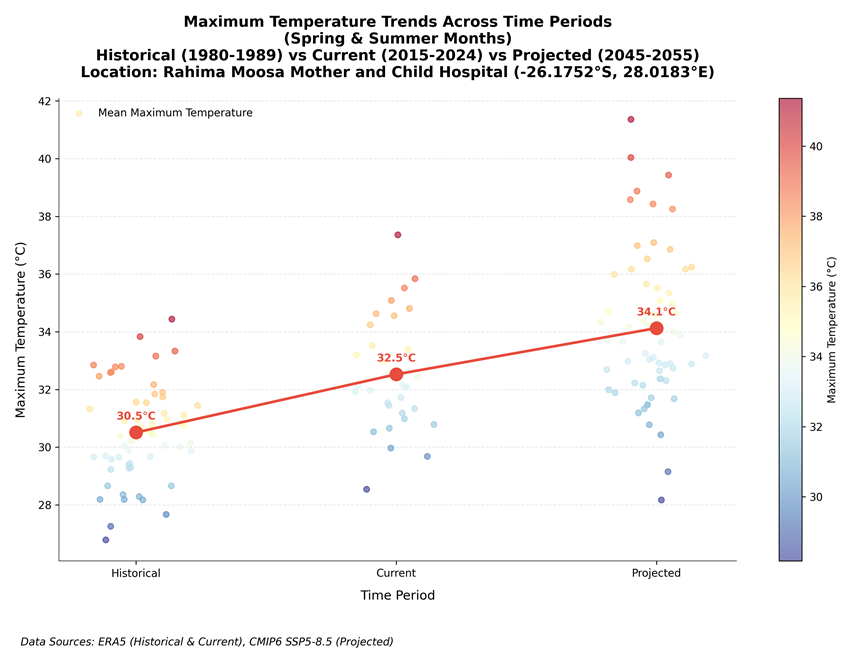
\includegraphics[width=0.7\textwidth]{sections/images/Max_temp_trends_across_time_periods.png}
    \caption{Maximum temperature trends across different time periods showing warming acceleration.}
    \label{fig:max_temp}
\end{figure}

\subsection*{F.2 Seasonal Heat Pattern Analysis}
\begin{figure}[H]
    \centering
    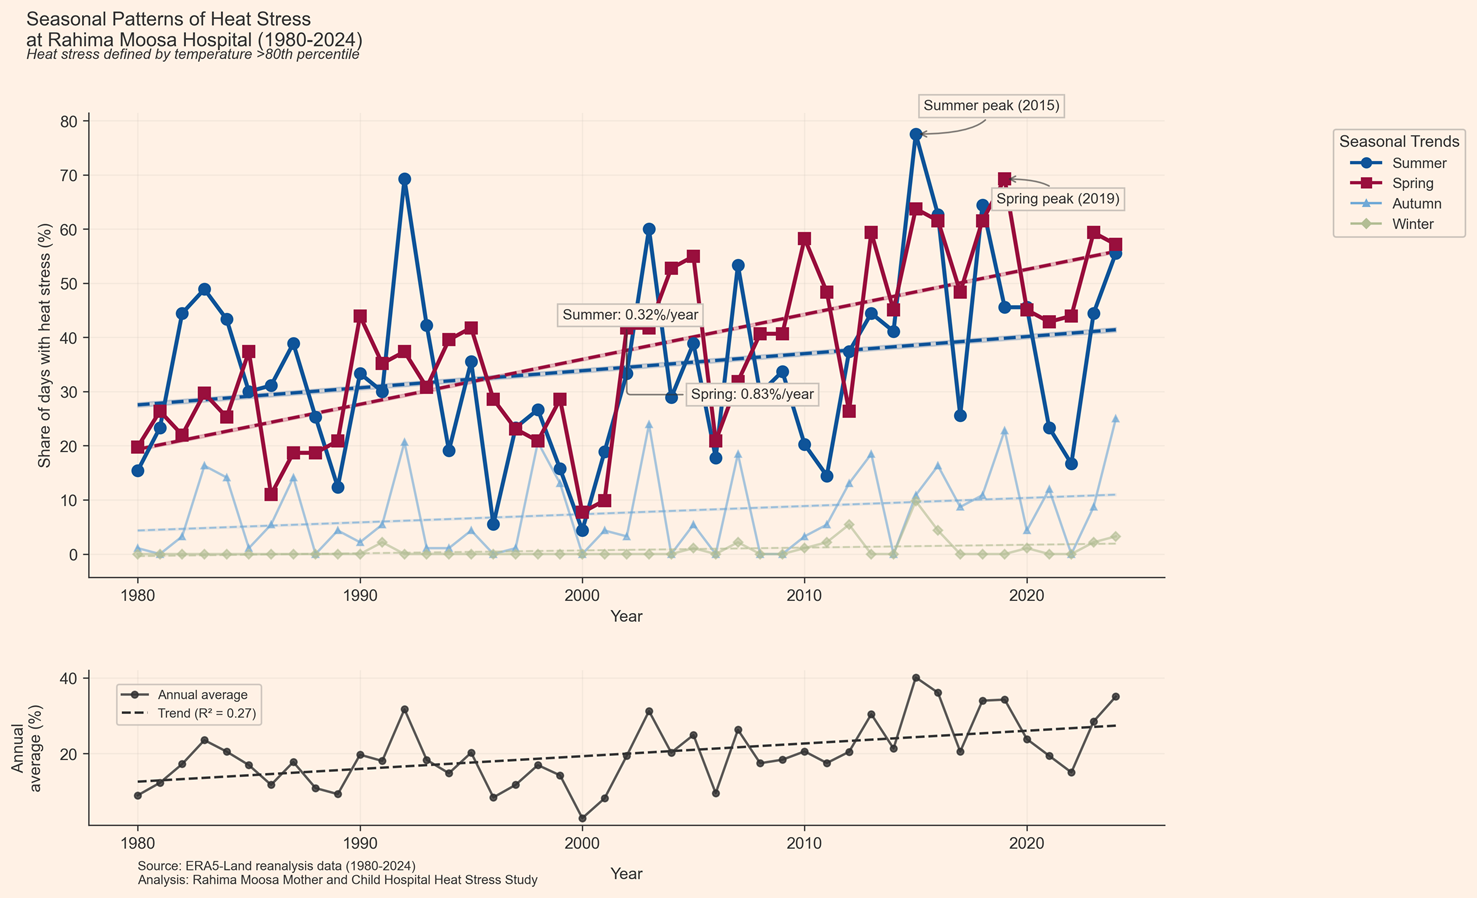
\includegraphics[width=0.7\textwidth]{sections/images/seasonal_heat_Rahima_1980_2024.png}
    \caption{Seasonal heat pattern variations across Johannesburg showing temporal vulnerability distributions.}
    \label{fig:seasonal}
\end{figure}

\subsection*{F.3 Global Temperature Trends}
\begin{figure}[H]
    \centering
    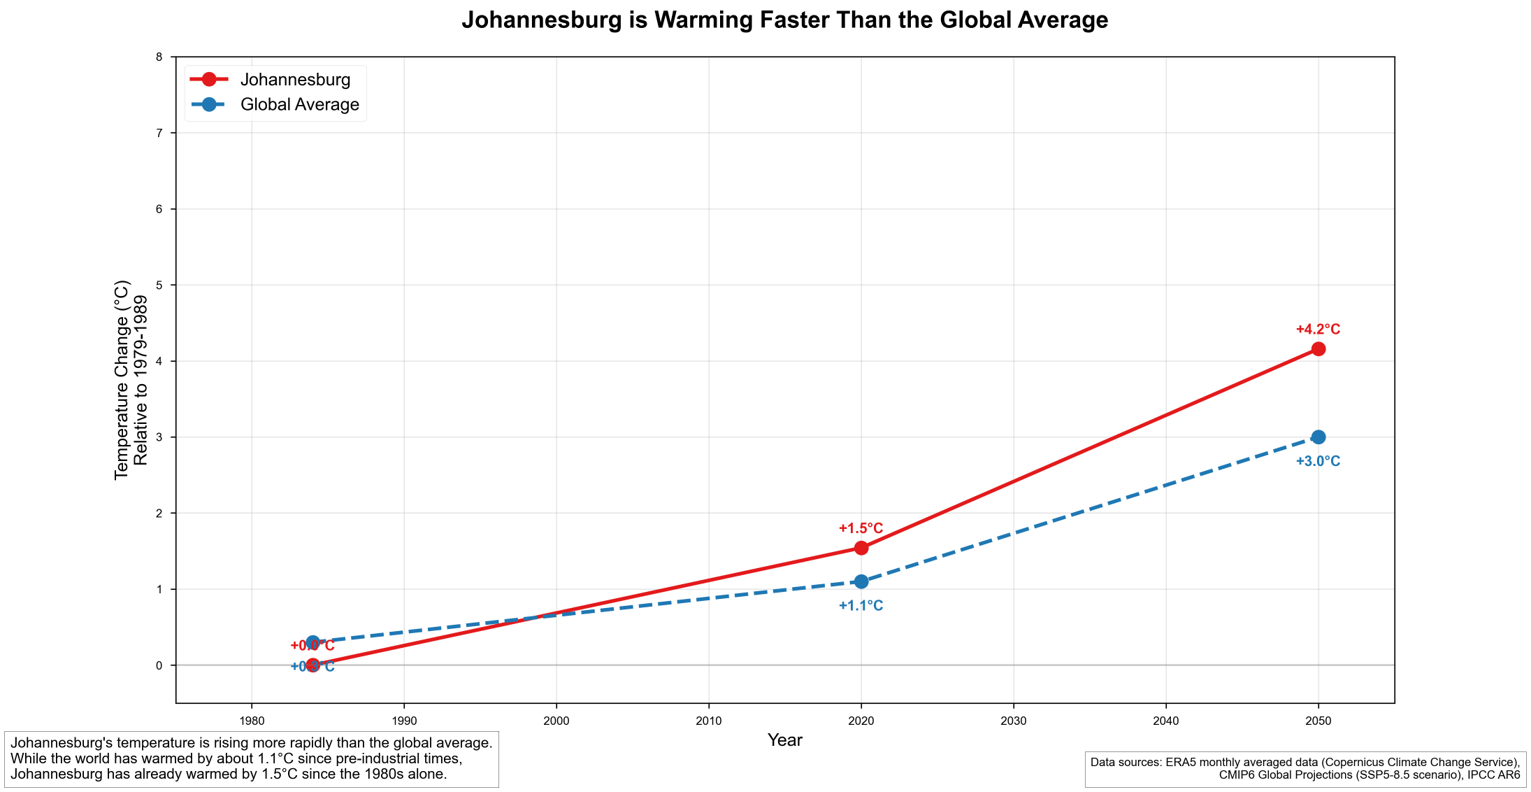
\includegraphics[width=0.7\textwidth]{sections/images/global_temp_versus_Johannesburg.png}
    \caption{Global temperature trends showing warming patterns relevant to urban heat studies.}
    \label{fig:global_temp}
\end{figure}

\subsection*{F.4 Urban Heat Stress Patterns}
\begin{figure}[H]
    \centering
    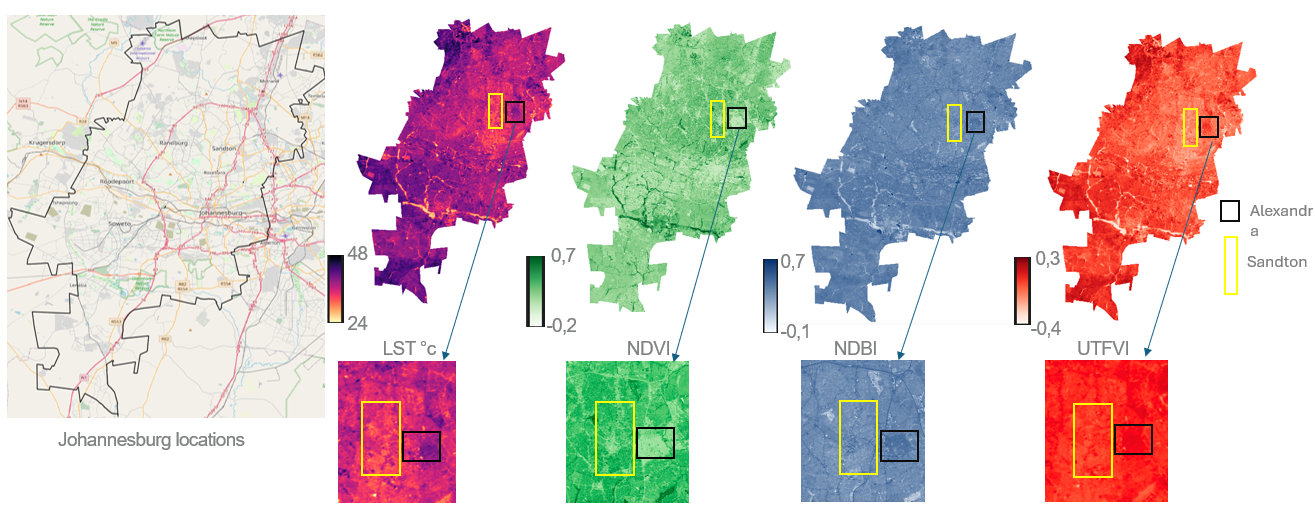
\includegraphics[width=0.7\textwidth]{sections/images/heat_stress_LST_NDVI_NDBI_UTFVI_Johannesburg.png}
    \caption{Visualization of heat stress patterns in urban environments with particular focus on informal settlements.}
    \label{fig:heat_stress}
\end{figure}

\subsection*{F.5 Heat Vulnerability Index Components}
\begin{figure}[H]
    \centering
    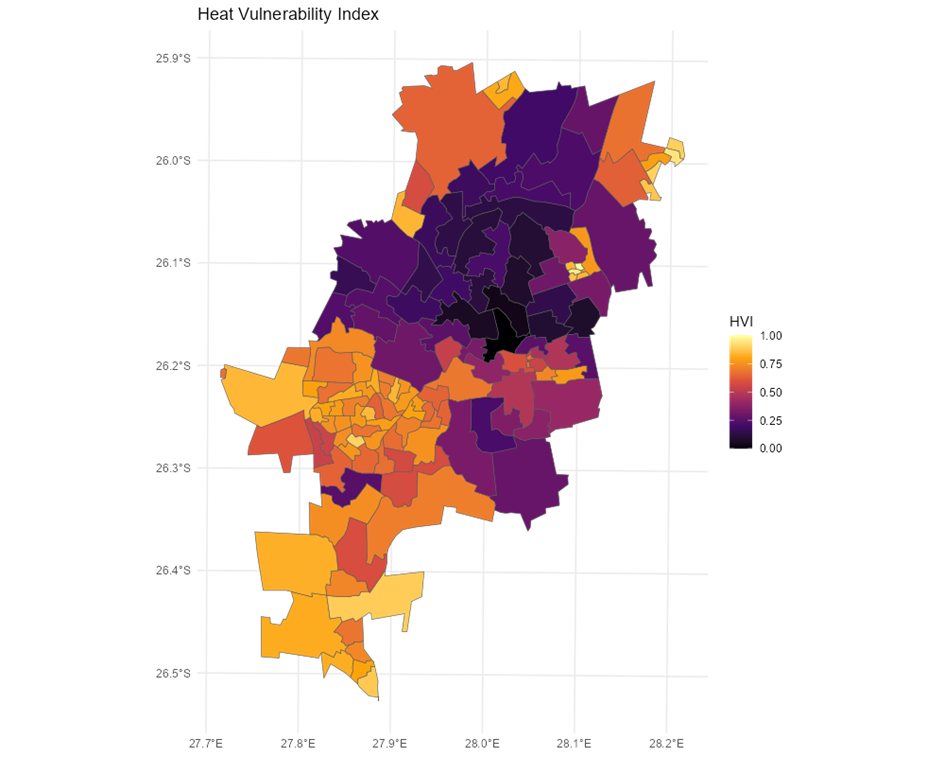
\includegraphics[width=0.7\textwidth]{sections/images/HVI_map_Johannesburg_prelim_analysis.png}
    \caption{Composite Heat Vulnerability Index (HVI) showing spatial distribution of vulnerability across Johannesburg.}
    \label{fig:hvi}
\end{figure}

\subsection*{F.6 Metabolic Pathway Analysis}
\begin{figure}[H]
    \centering
    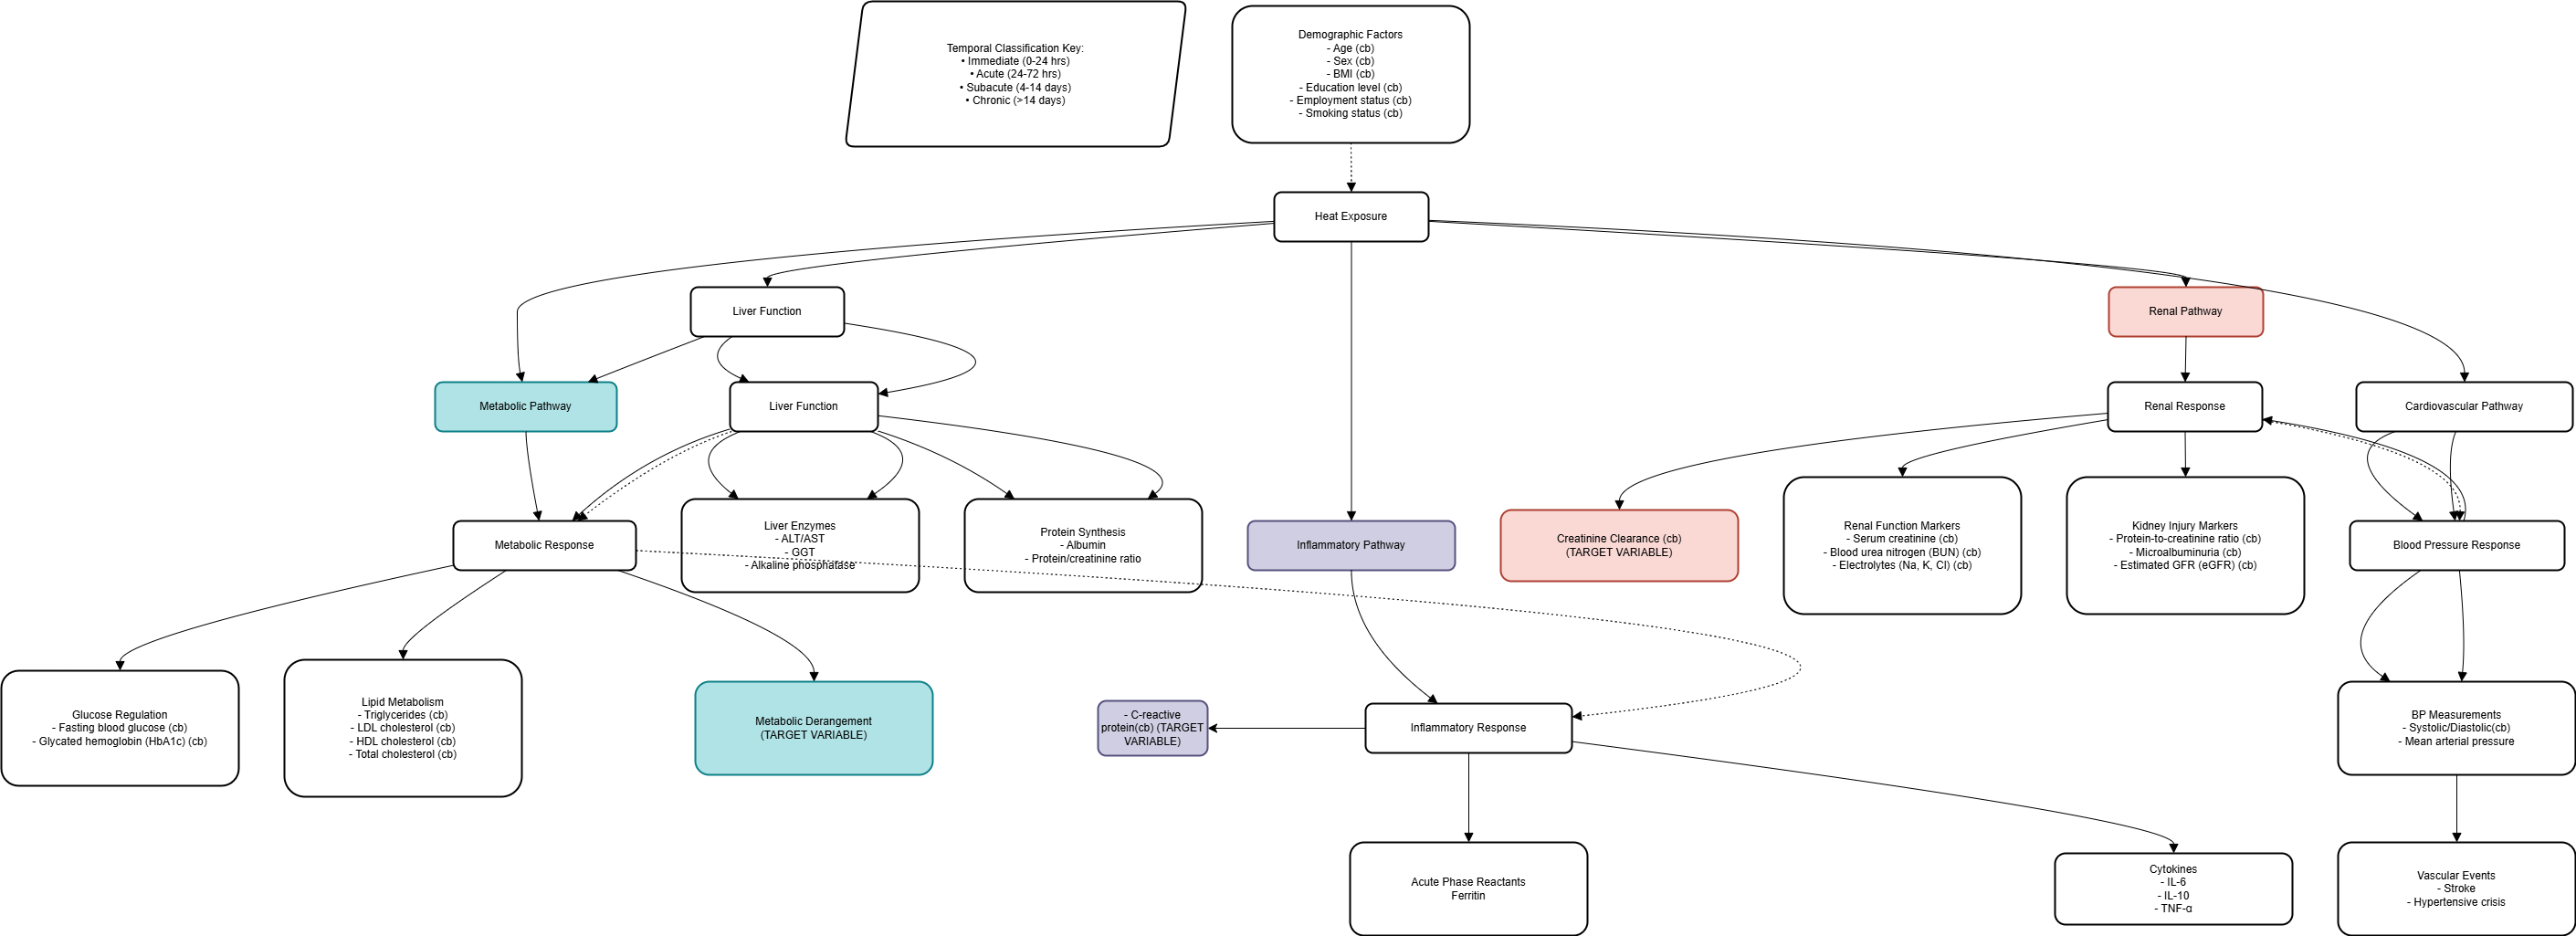
\includegraphics[width=0.7\textwidth]{sections/images/Timeline-Heat_health_mechanisms.drawio.png}
    \caption{Physiological pathways demonstrating heat impact on metabolic function and health outcomes.}
    \label{fig:metabolic}
\end{figure}

\subsection*{F.7 Inflammatory Mechanism Analysis}
\begin{figure}[H]
    \centering
    \includegraphics[width=0.7\textwidth]{sections/images/mechanisms-Inflammatory.drawio.png}
    \caption{Inflammatory pathways and mechanisms triggered by heat exposure showing systemic impacts.}
    \label{fig:inflammatory}
\end{figure}

\subsection*{F.8 Renal Mechanism Diagram}
\begin{figure}[H]
    \centering
    \includegraphics[width=0.7\textwidth]{sections/images/mechanisms-Renal.drawio.png}
    \caption{Detailed renal mechanisms affected by heat exposure and dehydration status.}
    \label{fig:renal}
\end{figure}

\begin{center}
    \Large\textbf{APPENDIX DOCUMENT}\\[0.5em]
    \normalsize\textit{The following tables and appendices are separated from the main document to support word count requirements.}
\end{center}

\section*{Data Management and Methodological Tables for HE\textsuperscript{2}AT Center Research}

%==================== Table 1 ====================
\subsection*{Table 1: Key Data Sources for Heat-Health Research}
\begin{longtable}{L{3cm}L{4cm}L{5cm}L{4cm}L{4cm}}
\toprule
\textbf{Data Category} & \textbf{Data Source} & \textbf{Description} & \textbf{Key Variables} & \textbf{Relevance} \\
\midrule
\endhead

\multirow{2}{*}{\textbf{Biomedical Data}} 
& Individual Participant Data Platform 
& Collation of prospectively collected high-quality data from pregnant women \& neonates 
& Preterm birth, pre-eclampsia, neonatal admission 
& Research on pregnant women and young children as high-risk populations \\
\cmidrule{2-5}
& HIV Databases 
& Pooled health database from cohorts and trials in Johannesburg, South Africa 
& Physical measurements, laboratory tests, health questionnaires 
& Study population with high rates of co-morbidities and adverse health outcomes \\
\midrule

\multirow{3}{*}{\textbf{Climate/Weather\\Data}} 
& ECMWF Forecasts 
& Outputs from numerical weather prediction system 
& Temperature, solar irradiance, wind speed, precipitation, pressure 
& Determination of heat hazard and thermal comfort metrics \\
\cmidrule{2-5}
& ERA5 Reanalysis 
& Global reanalysis dataset combining observed data with meteorological models 
& Temperature, wind speed, precipitation, atmospheric water content 
& Historical climate exposures assessment \\
\cmidrule{2-5}
& ERA5-Land 
& High-resolution land component of the ERA5 climate reanalysis 
& Surface temperature, precipitation, near-surface winds 
& Detailed land surface parameter analysis \\
\midrule

\multirow{3}{*}{\textbf{Remote Sensing\\Data}} 
& SRTM Elevation 
& Global elevation data (30m resolution) 
& Elevation 
& Urban heat island effect assessment \\
\cmidrule{2-5}
& Sentinel-2 Imagery 
& High-resolution multispectral satellite imagery 
& Vegetation coverage, land use classification, NDVI 
& Land cover and urban morphology analysis \\
\cmidrule{2-5}
& MODIS Land Surface Temperature 
& Daily global land surface temperature 
& Day/night land surface temperature 
& Heat exposure assessment \\
\midrule

\multirow{3}{*}{\textbf{Socio-Economic\\Data}} 
& Gauteng City-Region Observatory 
& GIS data for Gauteng City-Region 
& Demographics, economics, environmental factors 
& Socio-economic context for urban areas \\
\cmidrule{2-5}
& Quality of Life Surveys 
& Household survey data 
& Quality of life, socio-economic circumstances, service delivery attitudes 
& Vulnerability assessment inputs \\
\cmidrule{2-5}
& SEDAC Population Data 
& Global gridded population counts and densities 
& Population counts and density estimates 
& Population exposure quantification \\
\bottomrule
\caption{Key Data Sources for Heat-Health Research}
\end{longtable}
\clearpage

%==================== Table 2 ====================
\subsection*{Table 2: Data Processing and Integration Workflow}
\begin{longtable}{L{4cm}L{7cm}L{4cm}L{4.5cm}}
\toprule
\textbf{Processing Stage} & \textbf{Key Activities} & \textbf{Responsible Team} & \textbf{Outputs} \\
\midrule
\endhead

\textbf{Pre-processing} 
& Data reformatting, extraction of key variables, alignment with ontologies 
& Core Data Team 
& Standardized data formats ready for harmonization \\
\midrule

\textbf{Variable Mapping} 
& Mapping variables to standardized ontologies, using AI tools for suggestions 
& Harmonization Team 
& Consistent variable naming and definitions across datasets \\
\midrule

\textbf{Mapping Validation} 
& Cross-checking with original data, expert health review 
& Core Data Team, Health Experts 
& Validated variable mappings \\
\midrule

\textbf{Database Population} 
& Application of mappings, transformation of data, de-identification 
& Core Data Team 
& Integrated consortium-shared dataset \\
\midrule

\textbf{Climate Data Integration} 
& Automated retrieval of climate variables, spatial and temporal alignment 
& CSAG/UCT Team 
& Climate-integrated health dataset \\
\midrule

\textbf{De-identification} 
& Safe Harbor method application, expert determination, geographic aggregation 
& Core Data Team 
& RP2 De-identified datasets \\
\midrule

\textbf{Data Analysis} 
& Statistical analysis, machine learning applications 
& HE\textsuperscript{2}AT Consortium 
& Research outputs and inferential data \\
\bottomrule
\caption{Data Processing and Integration Workflow}
\end{longtable}
\clearpage

%==================== Table 3 ====================
\subsection*{Table 3: Data Access Levels and Security Measures}
\begin{longtable}{L{3.5cm}L{5cm}L{4.5cm}L{4cm}L{3cm}}
\toprule
\textbf{Data Level} & \textbf{Description} & \textbf{Access Permissions} & \textbf{Security Measures} & \textbf{Retention Period} \\
\midrule
\endhead

\textbf{Original Study Data} 
& Raw, unprocessed health data collected directly from studies 
& Core Data Team only 
& Encryption (AES-256), secure UCT servers, restricted access 
& 5 years after project completion \\
\midrule

\textbf{Consortium Shared Data} 
& Processed, harmonized data with limited indirect identifiers 
& HE\textsuperscript{2}AT Center Consortium partners 
& TLS protocols, access controls, authentication protocols 
& Indefinite (unless specified in DTA) \\
\midrule

\textbf{RP2 De-identified Data} 
& Further de-identified data with aggregated geographic information 
& External Bone Fide Researchers (DAC-approved) 
& Data Transfer Agreements, ethical approval requirements 
& Indefinite (unless specified in DTA) \\
\midrule

\textbf{Inferential Data} 
& Aggregated and anonymized data derived from analyses 
& Open access 
& NA - No identifying information 
& Indefinite \\
\bottomrule
\caption{Data Access Levels and Security Measures}
\end{longtable}
\clearpage

%==================== Table 4 ====================
\subsection*{Table 4: Geographic De-identification Techniques}
\begin{longtable}{L{4cm}L{6cm}L{6cm}L{4cm}}
\toprule
\textbf{Technique} & \textbf{Description} & \textbf{Application Scenario} & \textbf{Privacy Protection Level} \\
\midrule
\endhead

\textbf{Geographic Aggregation} 
& Aggregating addresses into larger regions 
& Areas with adequate population density 
& Medium - Depends on aggregation level \\
\midrule

\textbf{Random Direction and Fixed Radius} 
& Points displaced randomly within fixed radius 
& High spatial granularity needs 
& Medium - Predictable displacement bounds \\
\midrule

\textbf{Gaussian Displacement} 
& Random direction with distances following Gaussian distribution 
& Detailed spatial analysis requirements 
& High - Variable displacement with population density \\
\midrule

\textbf{Donut Masking} 
& Setting minimum and maximum displacement levels 
& Preventing both near and far relocations 
& High - Controls minimum displacement \\
\midrule

\textbf{K-anonymity Assessment} 
& Ensuring each location is indistinguishable from k-1 others 
& Validation of masking effectiveness 
& Verification mechanism \\
\bottomrule
\caption{Geographic De-identification Techniques}
\end{longtable}
\clearpage

%==================== Table 5 ====================
\subsection*{Table 5: Data Request and Approval Process}
\begin{longtable}{L{3.5cm}L{6cm}L{4.5cm}L{5.5cm}}
\toprule
\textbf{Stage} & \textbf{Description} & \textbf{Responsible Party} & \textbf{Key Considerations} \\
\midrule
\endhead

\textbf{Data Request Submission} 
& Completion of standardized form with research details 
& External Researcher 
& Research purposes, required datasets, ethics approval \\
\midrule

\textbf{Preliminary Screening} 
& Confirmation of form completeness and basic compliance 
& HE\textsuperscript{2}AT Center SteerCo 
& Resource availability, completeness of application \\
\midrule

\textbf{DAC Review} 
& Evaluation based on scientific, ethical, and feasibility criteria 
& Data Access Committee 
& Scientific merit, potential privacy risks, overlap with ongoing research \\
\midrule

\textbf{Decision Communication} 
& Documentation and notification of approval or rejection 
& DAC 
& Transparent reasoning, conditions for approval \\
\midrule

\textbf{Data Transfer} 
& Execution of DTA and data provision 
& Core Data Team 
& Secure transfer protocols, encryption \\
\midrule

\textbf{Ongoing Monitoring} 
& Regular reviews of compliance with agreement terms 
& DAC 
& Audits if necessary \\
\bottomrule
\caption{Data Request and Approval Process}
\end{longtable}

%==================== Table 6 ====================
\subsection*{Table 6: Methodological Approaches for Research Objectives}
\begin{table}[H]
\centering
\caption{Methodological Approaches for Research Objectives}
\label{tab:research_objectives}
\begin{tabular}{L{0.3\linewidth}L{0.6\linewidth}}
\toprule
\textbf{Objective} & \textbf{Methodological Approaches} \\
\midrule
\textbf{Vulnerability Mapping} & 
\begin{itemize}[leftmargin=*]
    \item Principal Component Analysis
    \item Geospatial analysis using GIS
    \item Satellite imagery integration
    \item Local Indicators of Spatial Association (LISA)
\end{itemize} \\
\midrule
\textbf{Heat-Health Dynamics} & 
\begin{itemize}[leftmargin=*]
    \item Random Forests for feature importance
    \item XGBoost with SHAP value interpretation
    \item Multi-scale time-series analysis
    \item Physiological pathway investigation
\end{itemize} \\
\midrule
\textbf{Predictive Modeling} & 
\begin{itemize}[leftmargin=*]
    \item Ensemble machine learning approaches
    \item Demographic stratification
    \item Advanced feature selection
    \item Time-series cross-validation
\end{itemize} \\
\bottomrule
\end{tabular}
\end{table}

%==================== Table 7 ====================
\subsection*{Table 7: Time-Lag Analysis of Heat-Health Effects}
\begin{table}[H]
\centering
\caption{Time-Lag Analysis of Heat-Health Effects}
\label{tab:time_lag}
\begin{tabular}{L{0.15\linewidth}L{0.35\linewidth}L{0.35\linewidth}}
\toprule
\textbf{Temporal Scale} & \textbf{Health Outcomes} & \textbf{Analytical Approach} \\
\midrule
\textbf{Immediate} \newline(0-24 hours) & 
\begin{itemize}[leftmargin=*]
    \item Cardiovascular responses
    \item Renal function markers
    \item Cognitive performance
\end{itemize} & 
\begin{itemize}[leftmargin=*]
    \item High-resolution temporal analysis
    \item Threshold identification
    \item Diurnal pattern examination
\end{itemize} \\
\midrule
\textbf{Short-term} \newline(1-7 days) & 
\begin{itemize}[leftmargin=*]
    \item Inflammatory markers
    \item Metabolic changes
    \item Sleep quality metrics
\end{itemize} & 
\begin{itemize}[leftmargin=*]
    \item Moving average analysis
    \item Cumulative exposure modeling
    \item Change-point detection
\end{itemize} \\
\midrule
\textbf{Medium-term} \newline(7-30 days) & 
\begin{itemize}[leftmargin=*]
    \item Chronic condition exacerbation
    \item Adaptation responses
    \item Cumulative health impacts
\end{itemize} & 
\begin{itemize}[leftmargin=*]
    \item Distributed lag models
    \item Trend analysis
    \item Physiological pathway assessment
\end{itemize} \\
\bottomrule
\end{tabular}
\end{table}

% Add clearpage after both tables
\clearpage

%--------------------------------------------------------------------------------
% APPENDIX A
%--------------------------------------------------------------------------------
\clearpage
\section*{Appendix A: Roles and Responsibilities in Data Management}

\begin{longtable}{L{3cm}L{6cm}L{5.5cm}L{5cm}}
\toprule
\textbf{Role} & \textbf{Responsibilities} & \textbf{Current Personnel} & \textbf{Contact} \\
\midrule
\endhead

\textbf{DMAC PIs} 
& Oversight of data management, plan assessment and updates 
& Christopher Jack (UCT), Sibusisiwe Makhanya (IBM) 
& cjack@csag.uct.ac.za, sibusisiwe.makhanya@ibm.com \\
\midrule

\textbf{Health Data Acquisition} 
& Identification of health datasets, DTA development 
& Craig Parker (RP2) 
& Craig.parker@witsphr.org \\
\midrule

\textbf{Core Data Team} 
& Data processing, de-identification, quality control 
& Lisa van Aardenne, Pierre Kloppers, Piotr Wolski, Peter Marsh, Nicholas Brink, Craig Parker 
& Contact DMAC PIs \\
\midrule

\textbf{Harmonization Team} 
& Variable mapping, integration, standardization 
& Core Data Team + consortium researchers 
& Contact DMAC PIs \\
\midrule

\textbf{Platform Access Management} 
& Managing access to analysis platforms 
& Rodger Duffett (UCT), Sibusisiwe Makhanya (IBM) 
& rodger@csag.uct.ac.za, sibusisiwe.makhanya@ibm.com \\
\bottomrule
\caption{Roles and Responsibilities in Data Management}
\end{longtable}

%--------------------------------------------------------------------------------
% POPIA Compliance
%--------------------------------------------------------------------------------
\clearpage
\section*{Appendix B: POPIA Compliance Framework}

\subsection*{B.2 POPIA Compliance Framework}

The research adheres to South Africa's Protection of Personal Information Act (POPIA, 2013) via:

\begin{enumerate}[leftmargin=*, itemsep=0.5em]
    \item \textbf{Lawful Processing}: All data processing is conducted exclusively for legitimate research purposes under POPIA Section 27.
    \item \textbf{Purpose Limitation}: Data is collected and processed solely for examining heat-health relationships and vulnerability patterns.
    \item \textbf{Data Minimization}: Only essential data elements required for valid scientific analysis are retained.
    \item \textbf{Information Officer Designation}: A designated Information Officer oversees POPIA compliance with quarterly audits.
    \item \textbf{Security Safeguards}: Includes AES-256 encryption, role-based access, multi-factor authentication, and regular security assessments.
    \item \textbf{Data Subject Participation}: Verification that original consent allows for secondary analyses, respecting broad consent principles.
    \item \textbf{Third-Party Processor Controls}: Data Transfer Agreements require POPIA compliance and verification.
\end{enumerate}

These measures ensure compliance with POPIA while enabling scientifically valid research benefiting public health.

%--------------------------------------------------------------------------------
% APPENDIX C
%--------------------------------------------------------------------------------
\clearpage
\section*{Appendix C: Detailed Project Timeline and Risk Assessment}

\subsection*{C.1 Comprehensive Timeline of Research Activities}
\begin{table}[H]
    \centering
    \caption{Comprehensive Project Timeline and Key Activities}
    \label{tab:timeline}
    \begin{tabular}{L{3cm}L{12cm}}
        \toprule
        \textbf{Timeline} & \textbf{Detailed Research Activities} \\
        \midrule
        Months 1-3 & Comprehensive literature review, protocol refinement, and ethics approval \\
        \addlinespace
        Months 4-9 & Systematic data collection and vulnerability mapping \\
        \addlinespace
        Months 10-18 & Advanced explanatory modeling \\
        \addlinespace
        Months 19-24 & Predictive model development and validation \\
        \addlinespace
        Months 25-30 & Validation studies and manuscript preparation \\
        \addlinespace
        Months 31-36 & Thesis writing and defense preparation \\
        \bottomrule
    \end{tabular}
\end{table}

\subsection*{C.2 Detailed Milestone Descriptions}

\begin{enumerate}[leftmargin=*, itemsep=0.5em]
    \item \textbf{Month 3: Protocol Development and Ethics Approval}
    \begin{itemize}[leftmargin=*]
        \item Comprehensive literature review on heat-health linkages
        \item Finalization of research protocol
        \item Submission and approval of ethics applications
        \item Establishment of data sharing agreements
    \end{itemize}
    
    \item \textbf{Month 9: Data Collection and Initial Analysis}
    \begin{itemize}[leftmargin=*]
        \item Acquisition of clinical trial datasets
        \item Harmonization of climate and health datasets
        \item Initial data preprocessing and quality assessment
        \item Preliminary exploratory data analysis
    \end{itemize}
    
    \item \textbf{Month 18: Vulnerability Mapping Completion}
    \begin{itemize}[leftmargin=*]
        \item Principal Component Analysis
        \item Development of composite vulnerability index
        \item Geospatial mapping of vulnerability distributions
        \item Local indicators of spatial association analysis
    \end{itemize}
    
    \item \textbf{Month 30: Model Development and Validation}
    \begin{itemize}[leftmargin=*]
        \item Explanatory modeling across diverse populations
        \item Predictive modeling with feature-importance analysis
        \item Time-series model validation
        \item Sensitivity analysis and model optimization
    \end{itemize}
    
    \item \textbf{Month 36: Thesis Completion and Submission}
    \begin{itemize}[leftmargin=*]
        \item Integration of research components
        \item Finalization of thesis
        \item Defense preparation
        \item Dissemination of findings
    \end{itemize}
\end{enumerate}

\subsection*{C.3 Risk Assessment and Contingency Planning}
\begin{table}[H]
    \centering
    \caption{Risk Assessment and Mitigation Strategies}
    \label{tab:risks}
    \begin{tabular}{L{3cm}L{6cm}L{6cm}}
        \toprule
        \textbf{Risk} & \textbf{Description} & \textbf{Mitigation Strategy} \\
        \midrule
        Data Accessibility & Limited clinical trial datasets & Expand data sources; maintain flexibility \\
        \addlinespace
        Computational Constraints & High-demand data processing & Leverage high-performance computing \\
        \addlinespace
        Pandemic Disruptions & COVID-19 research impacts & Stratify analysis across pandemic periods \\
        \addlinespace
        Model Performance & Predictive modeling challenges & Maintain methodological flexibility \\
        \bottomrule
    \end{tabular}
\end{table}

%--------------------------------------------------------------------------------
% APPENDIX D
%--------------------------------------------------------------------------------
\clearpage
\section*{Appendix D: Comprehensive Outcomes Impact Assessment and Dissemination Strategy}

\subsection*{D.1 Detailed Research Output Framework}
The research will produce four scholarly publications:

\begin{enumerate}[leftmargin=*, itemsep=0.5em]
    \item \textbf{Research Protocol Publication}
    \item \textbf{Vulnerability Analysis Publication}
    \item \textbf{Machine Learning Analysis Publication}
    \item \textbf{Predictive Models Publication}
\end{enumerate}

\subsection*{D.2 Extended Impact Assessment Framework}
\begin{table}[H]
    \centering
    \caption{Comprehensive Impact Assessment Framework}
    \label{tab:extended_impact}
    \begin{tabular}{L{2.5cm}L{5cm}L{5cm}L{3cm}}
        \toprule
        \textbf{Impact Domain} & \textbf{Primary Outcomes} & \textbf{Secondary Outcomes} & \textbf{Measurement Indicators} \\
        \midrule
        Public Health Practice & 
        Enhanced targeting of vulnerable populations; Improved intervention timing & 
        Reduced heat-related morbidity; More efficient resource allocation & 
        Heat-health outcome trends; Intervention cost-effectiveness \\
        \addlinespace
        Urban Planning & 
        Evidence-based cooling interventions; Prioritization of high-risk areas & 
        Improved thermal comfort; Enhanced greenspace distribution & 
        UHI intensity; Public space usage \\
        \addlinespace
        Policy Development & 
        Comprehensive heat-health action plans & 
        Increased cross-sector collaboration & 
        Policy adoption rates \\
        \addlinespace
        Climate Adaptation & 
        Holistic resilience strategies & 
        Improved adaptive capacity & 
        Vulnerability trend analysis \\
        \bottomrule
    \end{tabular}
\end{table}

\subsection*{D.3 Comprehensive Knowledge Dissemination Strategy}

\subsubsection*{D.3.1 Academic Dissemination}
\begin{itemize}[leftmargin=*]
    \item High-impact journals (e.g., \textit{The Lancet Planetary Health})
    \item Conferences (ISEE, Climate and Health Summit)
    \item Open-access data repositories
\end{itemize}

\subsubsection*{D.3.2 Policy Engagement}
\begin{itemize}[leftmargin=*]
    \item Tailored policy briefs
    \item Technical presentations to city planners
    \item Decision-support tools for health departments
\end{itemize}

\subsubsection*{D.3.3 Community and Public Engagement}
\begin{itemize}[leftmargin=*]
    \item Community workshops
    \item Accessible health protection guidance
    \item Collaboration with community health workers
\end{itemize}

\subsection*{D.4 Key Research Milestones and Quality Assurance}
\begin{table}[H]
    \centering
    \caption{Research Milestones and Quality Assurance Framework}
    \label{tab:milestones_qa}
    \begin{tabular}{L{3cm}L{6cm}L{6cm}}
        \toprule
        \textbf{Research Phase} & \textbf{Key Milestones} & \textbf{Quality Assurance} \\
        \midrule
        Initial Development & 
        Protocol finalization; Ethics approval & 
        Methodology review; Stakeholder needs \\
        \addlinespace
        Data Collection & 
        Data acquisition; Quality assessment & 
        Validation protocols; Documentation of limitations \\
        \addlinespace
        Analysis & 
        Vulnerability mapping; Model development & 
        Cross-validation; Sensitivity analyses \\
        \addlinespace
        Validation & 
        Model performance assessment & 
        Statistical validation; External review \\
        \addlinespace
        Dissemination & 
        Publications; Policy briefs & 
        Peer review; Policy relevance assessment \\
        \bottomrule
    \end{tabular}
\end{table}